\documentclass[11pt, A4paper]{article}
\usepackage[a4paper, total={7.2in, 10.5in}]{geometry}
\usepackage{tikz}
\usetikzlibrary{calc}
\usepackage{setspace}
\usepackage{graphicx}
\usepackage{amsmath}
\DeclareMathOperator\cis{cis}
\usepackage{pgfplots}
\graphicspath{ {./images/} }
\usepackage{bookmark}
\setcounter{tocdepth}{1}

%\usepackage[T1]{fontenc}
%\usepackage{mathptmx}

\hypersetup{
	colorlinks   = true, %Colours links instead of ugly boxes
	urlcolor     = blue, %Colour for external hyperlinks
	linkcolor    = black, %Colour of internal links
	citecolor   = red %Colour of citations
}

\newcommand{\tikzAngleOfLine}{\tikz@AngleOfLine}
\def\tikz@AngleOfLine(#1)(#2)#3{%
	\pgfmathanglebetweenpoints{%
		\pgfpointanchor{#1}{center}}{%
		\pgfpointanchor{#2}{center}}
	\pgfmathsetmacro{#3}{\pgfmathresult}%
}

\title{Further Mechanics Notes}
\author{Xingzhi Lu}

\begin{document}
	\maketitle
	\section{Momentum and impulse}
	\subsection{Equations}
	\begin{description}
		\item[Momentum:] $p=mv$ (unit=$kg \: ms^{-1}$)
		\item[Impulse:] $I=\Delta mv=mv-mu=Ft$ (unit=$Ns$)
	\end{description}
	
	\subsection{Conservation of momentum}
	\begin{itemize}
		\item Momentum is always conserved in any interaction where no external forces act
		\item Elastic collision: $m_1u_1+m_2u_2=m_1v_1+m_2v_2$
		\item Sticking together: $m_1u_1+m_2u_2=(m_1+m_2)v_{1+2}$
		\item Explosion: $m_1v_1+m_2v_2=0$
	\end{itemize}
	
	\subsection{Momentum as a vector}
	Calculate each direction independently
	
	
	
	\section{Work, energy and power}
	\subsection{Work and energy}
	\begin{description}
		\item[Work done:] $w=Fd=\text{force}\times\text{distance moved in the direction of the force}=\text{change in kinetic energy}$
		\item[Kinetic energy:] $\text{K.E.}=\dfrac{1}{2}mv^2$
		\item[Potential energy:] $\text{P.E.}=mgh$
	\end{description}
	\subsubsection{Calculating PE}
	\begin{itemize}
		\item You must choose a zero level of potential energy before calculating a particle's potential energy
		\item Take $g=9.8 ms^{-2}$
	\end{itemize}
	
	
	\subsection{Conservation of mechanical energy}
	When no external forces (other than gravity) do work on a particle during its motion, the sum of the particle's \textbf{kinetic energy and (gravitational and potential) potential energy} remains constant
	
	\subsection{Work-energy principle}
	The change in the total energy of a particle is equal to the work done on the particle
	
	\subsection{Power}
	\begin{description}
		\item[Definition:] Power is the rate of doing work
		\item[Equation:] $\text{Power}=Fv=\text{driving force produced by the engine}\times\text{velocity}=\text{the rate of work being done}$
	\end{description}
	
	\section{Elastic strings and springs and elastic energy}
	\subsection{Hooke's law}
	\begin{itemize}
		\item $\text{Tension produced}\propto x$ $\rightarrow$ $T=kx$, where $k$ is a constant
		\item $k$ depends on the unstretched length of the string or spring ($l$) and the \textbf{modulus of elasticity of the string or spring} ($\lambda$, unit=$N$)
		\item Hence $T=\dfrac{\lambda x}{l}$
		\item[*] Can also be applied if the string or spring is compressed
	\end{itemize}
	
	\subsection{Elastic energy}
	\begin{itemize}
		\item Work done in stretching an elastic string or spring of modulus of elasticity $\lambda$ from its natural length $l$ to a length of $(l+x)$ = $\dfrac{\lambda x^2}{2l}$
		\item Elastic potential energy stored = amount of energy used to stretch the spring = $(l+x)$ = $\dfrac{1}{2}kx$ = $\dfrac{\lambda x^2}{2l}$
		\item[*] Can also be applied when an elastic string or spring is compressed
	\end{itemize}
	
	
	\section{Elastic collisions in one dimension}
	\subsection{Newton's law of restitution}
	\begin{description}
		\item[Particles colliding:] $e=\dfrac{\text{speed of separation of particles}}{\text{speed of approach of particles}}$
		\item[Direct collision with a smooth plane:] $e=\dfrac{\text{speed of rebound}}{\text{speed of approach}}$
		\item[Range:] $0 \leq e \leq 1$
	\end{description}
	
	\subsection{Loss of kinetic energy}
	Loss of kinetic energy due to impact = $(\dfrac{1}{2}m_1u_1^2+\dfrac{1}{2}m_2u_2^2)-(\dfrac{1}{2}m_1v_1^2+\dfrac{1}{2}m_2v_2^2)$
	
	\subsection{Problems with modelling}
	\begin{description}
		\item[Bouncing for an infinite number of times:] the ball should stop bouncing after a finite number of bounces
		\item[Spheres modelled as particles:] air resistance is ignored
	\end{description}
	
	\section{Elastic collisions in two dimensions}
	\subsection{Oblique impact with a fixed surface}
	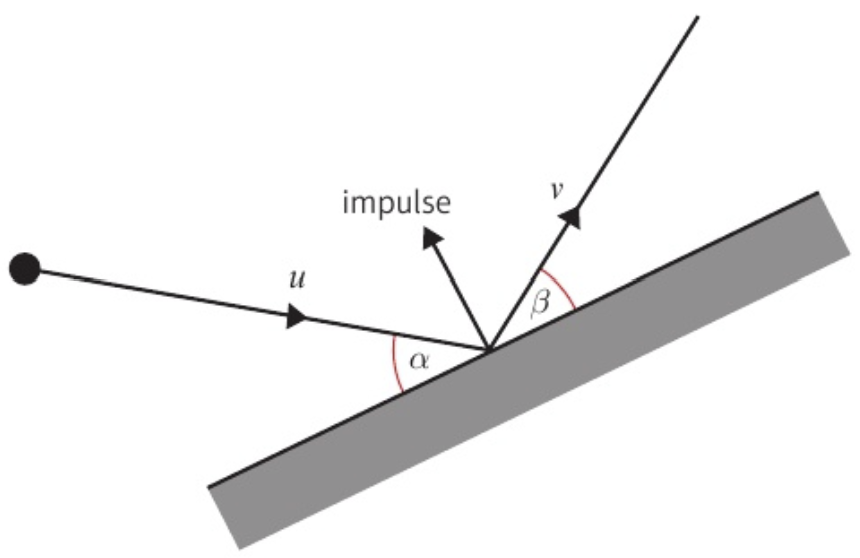
\includegraphics[width=0.3\textwidth]{obliqueimpact}
	\begin{itemize}
		\item The component of the velocity of the sphere parallel to the surface is unchanged: $v\cos\beta = u\cos\alpha$
		\item The component of the velocity of the sphere perpendicular to the surface can be found with Newton's law of restitution: $v\sin\beta = eu\sin\alpha$
		\item Hence $\tan\beta = e\tan\alpha$, since $0 \leq e \leq 1$, $\beta \leq \alpha$
		\item $\text{Loss of kinetic energy}=\dfrac{1}{2}mu^2-\dfrac{1}{2}mv^2$
	\end{itemize}
	\subsection{Oblique impact of smooth spheres}
	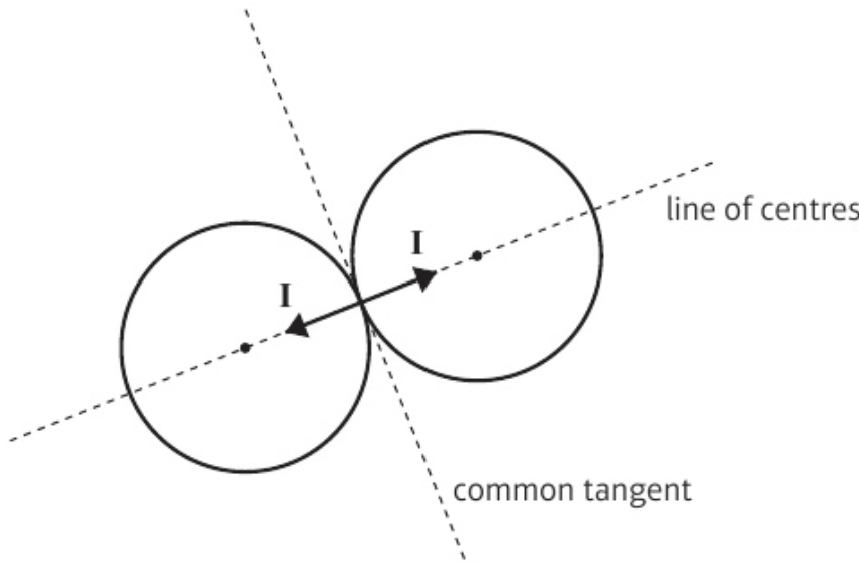
\includegraphics[width=0.3\textwidth]{oblique_2_balls}
	\begin{itemize}
		\item Impulse affecting each sphere acts along the line of centres
		\item The components of the velocities of the spheres \textbf{perpendicular}  to the line of centres are unchanged in the impact
		\item The principle of conservation of momentum and Newton's law of restitution applies \textbf{parallel} to the line of centres
	\end{itemize}
	
	
	
	
	
\end{document}